%%%%%%%%%%%%%%%%%%%%%%%%%%%%%%%%%%%%%%%%%%%%%%%%%%%%%%%%%%%%%%%%%%%
% Background
% Team:
% Wolverine
% Members: 
% Eric Lee, Jacky Wu, Karthick Mani, 
% Eric Chang, Dexter Chen, Peter Chen
% Relative files:
% Team_Wolverine.tex, Team_Wolverine_Compile.tex, Library.bib, WolverineChart.png
% Note:    
% Do not compile this file compile Main.tex to get the pdf file instead.
%%%%%%%%%%%%%%%%%%%%%%%%%%%%%%%%%%%%%%%%%%%%%%%%%%%%%%%%%%%%%%%%%%%
	
\subsection{Information retrieval of existing database}
Author: Eric Lee, Jacky Wu, Karthick Mani, Eric Chang, Dexter Chen, Peter Chen, Kenvin Lo

We live in the time that technologies evolved at a speed that we can't imagine. Due to rapidly increasing amount of informations, we can't use traditional ways to store data. With such a large amount of informations. We need to create a database that can store these data, more importantly a database that can allow us to easily find the informations we want easily.

A database management system (DBMS) is a computer software application that interacts with the user, other applications, and the database itself to capture and analyze data. Well-known DBMSs include MySQL, PostgreSQL, Microsoft SQL Server, Oracle, Sybase and IBM DB2. And they can support different kinds of databases.

Same as Relational database, object oriented database management systems was developed during 1970s. Db4o which was launched in 2004 represents an object oriented database model. It provides an easy interface to work for object oriented programming languages. And it also includes various object oriented programming language. For this reason, the programmer can work in one environment persistently. Here are the advantages and disadvantages of the three kinds of databases mentioned above.

\paragraph{1. Object-oriented database}
An object-oriented database (OODBMS) is a kind of database management 	system.\cite{WiKiauthor2013} The information in the database is represented as objects as used in object-oriented programming.

Because of the tighter integration with object-oriented language, the programmer is easier to maintain consistency with the same representation in both OODBMS and programing language.

Although relational databases which is table-oriented might be similar to object-oriented databases, But they are actually different. Object-oriented database supports objects, classes and inheritance in database schemes and query language.
There are many advantages for OODBMS compared to relational database management system(RODBMS) such as the performance, flexibility, and development cost.

And OODBMS also have some disadvantages, the \cite{Systems2010} have mention 3 disadvantage for OODBMS. First, because the usage is forced to be similar with object-oriented language. This make maintaining and evolving is  difficult. Second, the technique for store complex type of information take additional computational resources. Third, lack of a standard data model leads to design errors and inconsistencies.


\paragraph{2. Relational database}
A relational database is the most popular database used in the world. They can organize data into one or more tables of columns and rows, with a unique key identifying each row. Rows are also called records or tuples. Generally, each table represents one "entity type" (such as customer or product). The rows represent instances of that type of entity (such as "Lee" or "iPhone 6") and the columns representing values attributed to that instance (such as address or price).

Because of the method of the organization of data, relational database is much easier to understand and is flexible for you to manipulate the data. Besides SQL is easy in the relational database approach. For data organized in other structure the query language either becomes complex or extremely limited in its capabilities. However, once the attributes of data become more and more, you'll need a large amount of table to store your information. Therefore, the performance of relational database will decrease obviously.


\paragraph{3. Graph database}
Graph database uses graph structures for semantic queries with nodes,  edges and properties to represent and store data. Most graph databases are NoSQL in nature and store their data in a key-value store or document-oriented database. Graph databases are a powerful tool for graph-like queries, for example computing the shortest path between two nodes in the graph. Other graph-like queries can be performed over a graph database in a natural way.

Compare to relational databases, there are several advantages. Graph database are often faster for associative data set and map more directly to the structure of object-oriented applications. They can scale more naturally to large data sets as they do not typically require expensive join operations. As they depend less on a rigid schema, they are more suitable to manage ad hoc and changing data with evolving schema.

And graph database have also some disadvantages, relational database are typically faster at performing the same operation on large numbers of data elements. Finally, we want to take one example of graph database: AllegroGraph. 

Because of our lack of the experience of building a database, we think it is important for us to choose a database which is easy to learn and convenience to solve problems we may encounter. Furthermore, it seems relational database is the most capable database which can handle large data among them. Therefore, relational database is our choice.\\


According to many database website and discussion thread, there are many method to store a binary data with a database. The two main directions is store in the database and store out of the database. I will always be suggested not to store binary data in database if the binary is large. That will cause significant performance decrease and additional storage space. And another way is to store binary data in file system, and record the path in the database, that will not cause performance decrease when large binary data. But the binary data cannot automatic distributed with the database. Even the PDF document is not a large data, but still cost some performance. And our system have no requirement to automatic distribute. Our suggest for store PDF document is storing in the file system.

\begin{figure*}[h]
	\begin{center}
		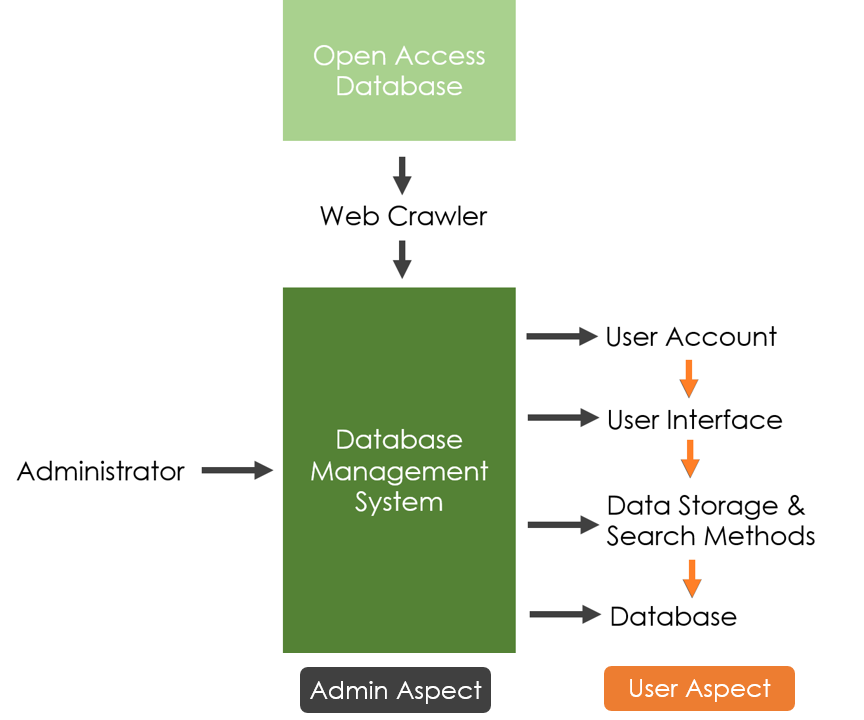
\includegraphics[scale=0.4]{WolverineChart}
	\end{center}
	\caption{Structure of our system}
	\begin{center}
		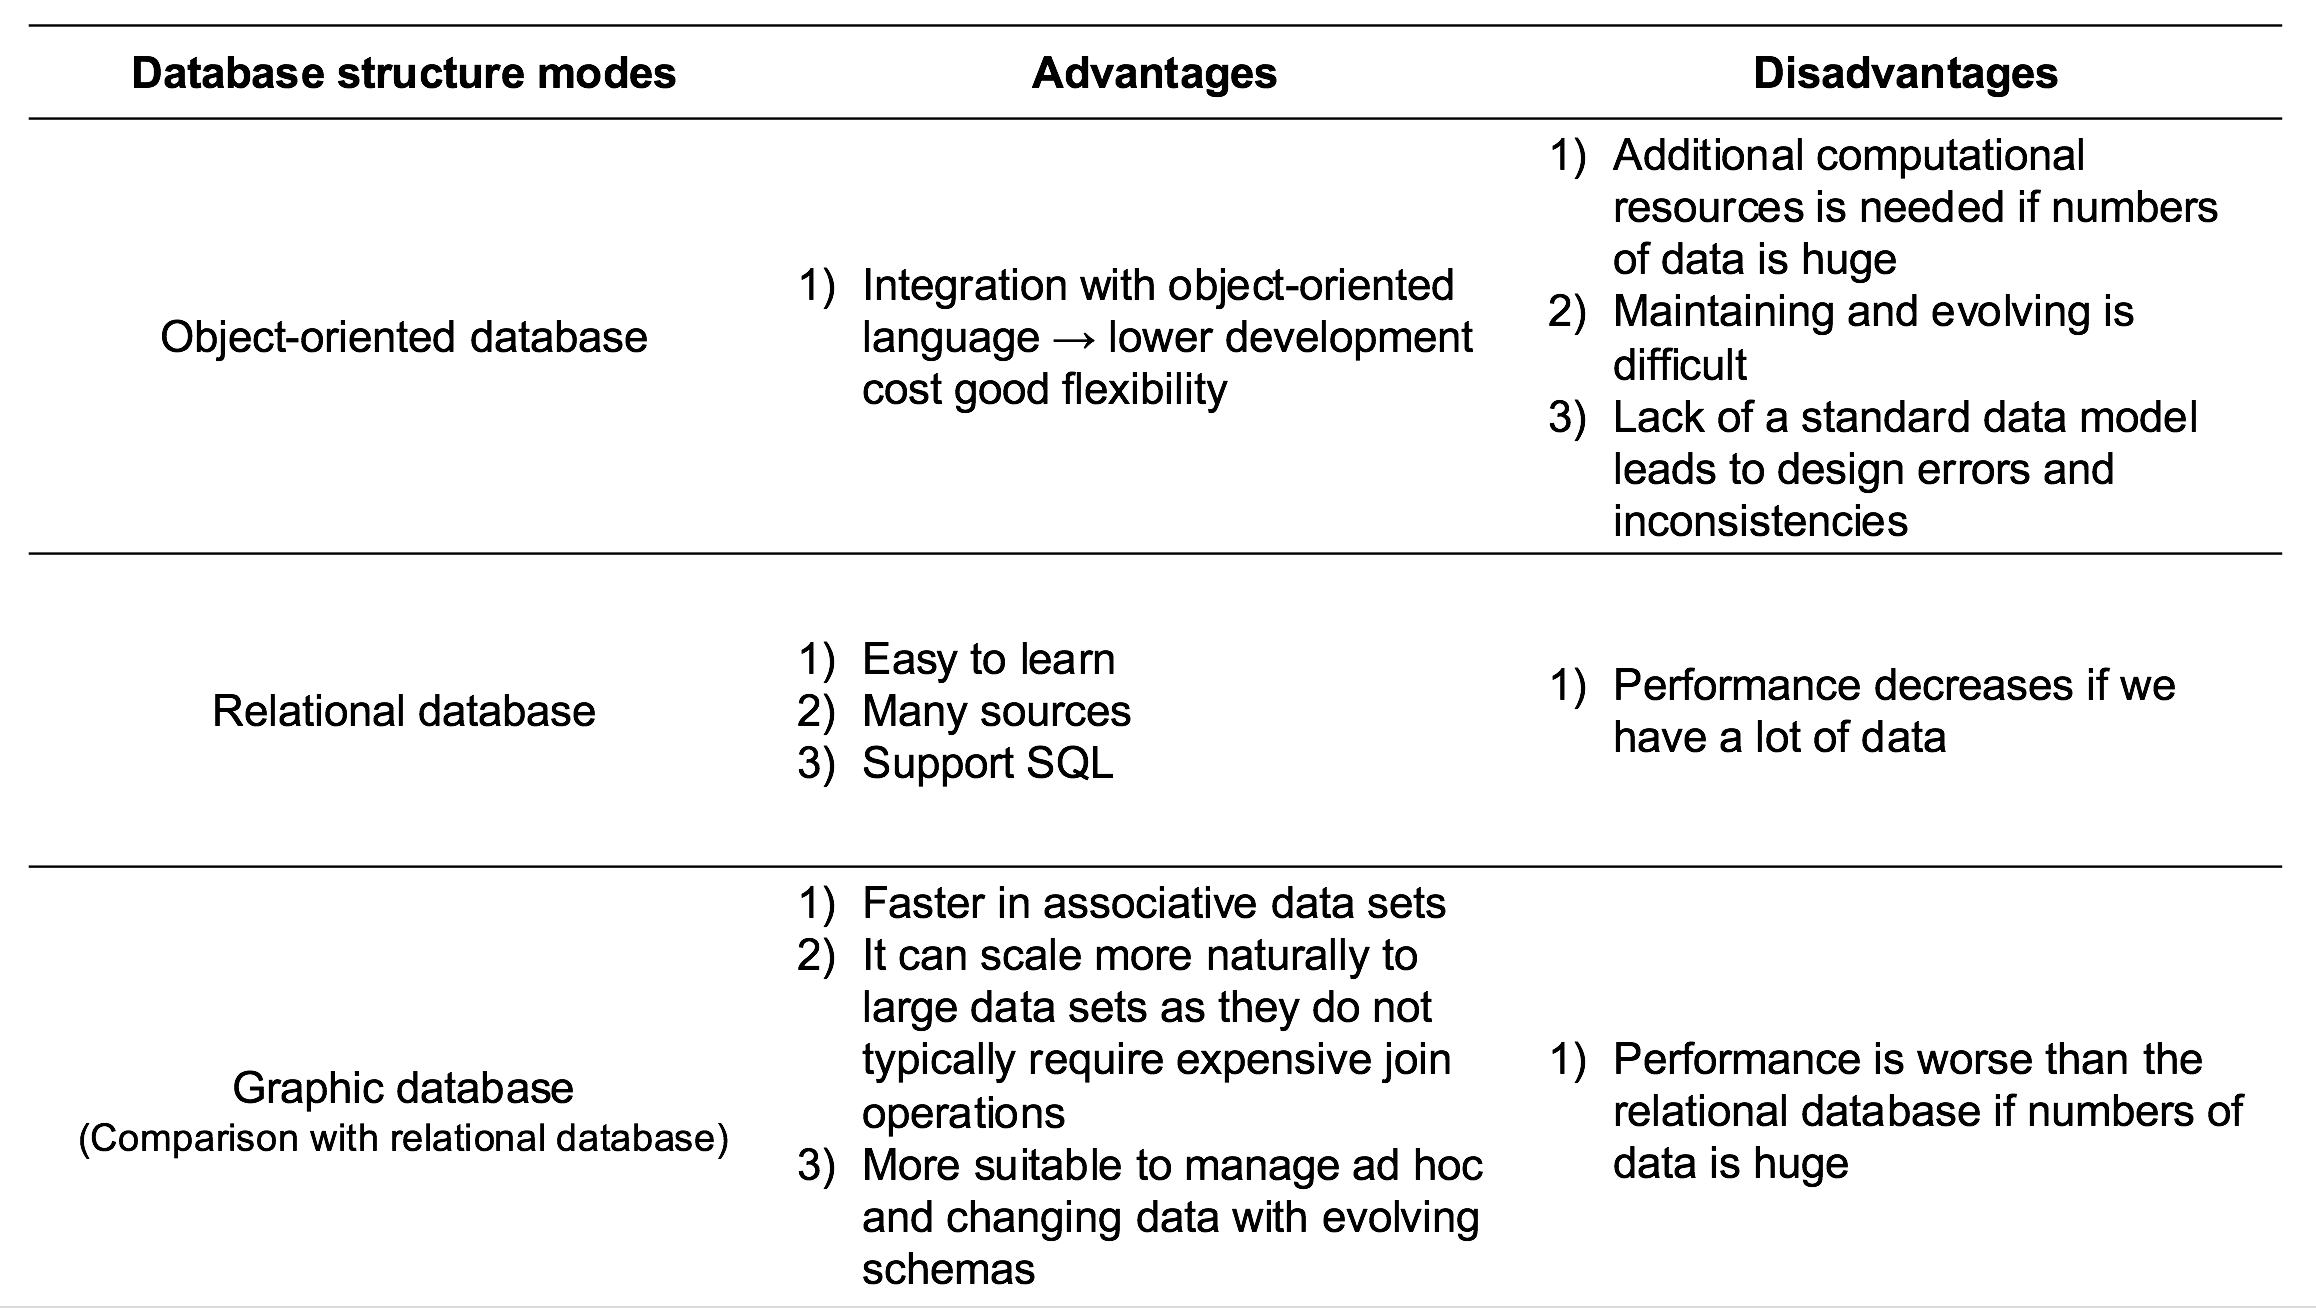
\includegraphics[scale=0.3]{WolverineChart2}
	\end{center}
	\caption{Database structure modes}
\end{figure*}
\clearpage
